\chapter{Анализ физических ограничений для решения задачи в ординарных и двойных каскадах}\label{ch:ch2}

Как уже было отмечено в главе \ref{ch1}, лишь некоторые из предложенных к настоящему моменту способов обогащения регенерированного урана потенциально способны решить задачу обогащения регенерата произвольного исходного состава в условиях одновременного выполнения ограничений на концентрации сразу нескольких изотопов и при заданном отношении между массой получаемого НОУ и исходной смеси регенерированного урана, поступающего для обогащения. В первую очередь, это касается разбавляющих схем на основе ординарного каскада. 
Однако, проведенный в главе \ref{ch1} теоретический анализ не позволяет априори определить при каких условиях может быть применена та или иная схема. В рамках настоящей главы кратко представлены результаты вычислительных экспериментов и сопутствующего им теоретического анализа, направленных на выявление области возможного применения одиночных каскадных схем с разбавлением и двойных каскадов для получения обогащенного регенерированного урана в условиях многократного рецикла. 

\section{Постановка задачи и методическая часть}\label{ch2_stat}

Рассмотрим модификации каскадов для обогащения регенерированного урана с одновременным его разбавлением несодержащим четных изотопов материалами, основанные на ординарном каскаде (рисунок \ref{fig:diagram1}). Каждая из схем, представленных на рисунке \ref{fig:diagram1} реализует один из возможных способов разбавления регенерированного урана. Отличия в способах состоят в том, в каком именно узле осуществляют разбавление регенерата, либо в том, что используют в качестве разбавителя (например, природный уран или НОУ из природного сырья).


Вставить новый рисунок со схемами и обозначенными потоками 



Основная цель описанных ниже вычислительных экспериментов -- оценить возможности рассматриваемых вариантов каскадов для обогащения регенерированного урана в условиях заметных (до одного порядка) колебаний изотопного состава регенерата, что характерно для его многократного рецикла. Для этого рассмотрены случаи обогащения регенерированного урана двух составов с различным исходным содержанием чётных изотопов (см. таблицу \ref{is_compositions_2_5}). Выбранные составы отвечают регенерированному урану, выделенному из ОЯТ реакторов ВВЭР-1000 и -1200 при различных внешних условиях \cite{palkinDesignanalyticalResearchRefinement2010,nevinicaToplivnyyCiklLegkovodnogo2019}. Отметим, что оба состава характеризуются высоким содержанием $^{232}$U, которое превышает предельно допустимый уровень концентарции $^{232}$U в конечном НОУ-продукте (например, $5\cdot10^{-7}$\%). Выбор подобных загрязненных четными изотопами составов регенерата имитирует сложности, которые могут возникать при обогащении регенерированного урана в условиях его многократного рецикла.  
При реализации вычислительных экспериментов общая постановка задачи соответствовала формулировке, приведенной в Главе \ref{ch1}. С учётом конкретных выбранных ограничений ее можно представить в следующем виде.

Из заданной массы исходного регенерированного урана необходимо получить заданную массу товарного НОУ, отвечающего следующим требованиям:

\begin{enumerate}
  \item Концентрация в конечном продукте составляет 4,95\%, значение характерно для современных легководных реакторов \cite{solovevaCennostiOYaTKak2019}.
  \item Расход регенерированного урана на единицу конечного продукта в виде низкообогащенного урана: 0,93 кг на 1 кг НОУ \cite{smirnovApplyingEnrichmentCapacities2018}.
  \item Концентрация $^{235}$U в потоке отвала задана равной 0,1\% \cite{smirnovEvolutionIsotopicComposition2012};
  \item Соотношение $^{234}$U к $^{235}$U не должно превышать значения 0,02.
  \item Влияние изотопа $^{236}$U на нейтронно-физические характеристики топлива должно быть скомпенсировано дополнительным обогащение по $^{235}$U, для расчёта которого коэффициент компенсации реактивности принят равным 0,29 \cite{smirnovApplyingEnrichmentCapacities2018}.
  \item Концентрация $^{232}$U ограничена величиной $5\cdot10^{-7}$\% \cite{smirnovApplyingEnrichmentCapacities2018}.
\end{enumerate}

Решение подобной задачи означает поиск такого набора параметров каждой из представленных на рисунке \ref{fig:diagram1} схем, который обеспечит одновременное удовлетворение перечисленных выше условий. Как следует из анализа рисунка, каждая из схем подразумевает использование ординарного каскада, которые обогащает либо регенерированный уран, либо природный в зависимости от выбранного способа. Остальные параметры рассчитывают на основе выбора отношения между смешиваемыми потоками и заданного состава разбавителя. Это означает, что для моделирования процеса обогащения урана в каскаде достаточно использования какой-либо модели ординарного каскада. В рамках работы была выбрана модель R-каскада \cite{sulaberidzeTeoriyaKaskadovDlya2011}. При этом для всех рассматриваемых схем при расчёте параметров каскада задавали концентрации $^{235}$U в его внешних выходящих потоках. Таким образом, расчёт параметров такого каскада был сведен к ранее рассмотренной задаче проектировочного расчета и подразумевал следующую математическую постановку задачи. 

Задано: 

концентрации компонентов исходной смеси регенерированного урана -- ${C}_{i,F}$; коэффициент разделения для единочной разности массовых чисел одиночного разделительного элемента -- ${q}_{0}$ ; величина одного из внешних потоков каскада, например, P или F; концентрации $^{235}$U в потоках отбора и отвала каскада -- {(C_{235, P})}, {(C_{235, W})}; номера компонентов, для которых выполнено условие несмешивания по относительным концентрациям -- n и к.
В процессе расчёта необходимо определить следующие параметры: 

величины N и f; концентрации ${C}_{i,W}$ и ${C}_{i,P}$ ($i \neq n$U, где индекс n соответствует $^{235}$U) в выходящих из каскада потоках; отношения внешних потоков каскада -- $P/F$, $W/F$; распределения потока и концентраций компонентов по ступеням каскада -- $L_{s}$, $C_{i,s}$; значения срезов потоков на ступенях -- $\theta_{s}$; остальные внутренние параметры каскада. 
Описанная постановка задачи расчета параметров ординарного R-каскада требует численного решения системы нелинейных уравнений, из которых возможно определить величины N и f, отвечающие заданным значениям концентраций целевого компонента во внешних потоках (см. раздел...) . Указанная система может быть записана в следующем виде: 

\begin{equation}
  \begin{cases}
  \Delta_{P} = {(C_{235, P})}_{calc}-{(C_{235, P})}_{given}\\
  \Delta_{W} = {(C_{235, W})}_{calc}-{(C_{235, W})}_{given}
  \end{cases}\,
\end{equation}

, где ${(C_{235, P})}_{calc}$, ${(C_{235, W})}_{calc}$ -- рассчитанные концентрации $^{235}$U в потоках отбора и отвала каскада, соответственно; ${(C_{235, P})}_{given}$, ${(C_{235, W})}_{given}$ -- заданные концентрации $^{235}$U в потоках отбора и отвала каскада, соответственно; а $\delta_{P}$, $\delta_{W}$ -- невязки по $C_{235, P}$ и $C_{235, W}$, соответственно. 

В случае использования модели R-каскада в указанных выше уравнениях удобно использовать соотношения (\ref{GrindEQ__1_72_}), (\ref{GrindEQ__1_73_}). В этом случае из решения системы определяют величины $R_{n k}^{W}$ и $R_{n k}^{P}$, после чего аналитически рассчитать остальные внешние параметры R-каскада по соотношениям (\ref{GrindEQ__1_70_})-(\ref{GrindEQ__1_77_}), а также непосредственно определить рассчитать N и f.   

\begin{table}[h]
  \centering
  \normalsize\begin{tabulary}{1.0\textwidth}{|c|c|c|c|c|c|c|}
  \hline Состав № & Массовое число & 232 & 233 & 234 & 235 & 236 \\
  \hline 1 & C, \% & $6,62\cdot10^{-7}$ & $1,19\cdot10^{-6}$ & $3,28\cdot10^{-2}$ & 1,43 & 0,9932 \\
  2 & C, \% &  $1,03\cdot10^{-6}$ & $1,3\cdot10^{-6}$ & $3,91\cdot10^{-2}$ & 1,07 & 1,45 \\\hline
  \end{tabulary}
  \caption{{Изотопные составы регенерата различных циклов.{\label{is_compositions_2_5}}}}
\end{table}

Ниже представлены результаты моделирования обогащения регенерата в каждой из трёх схем, представленных на рисунке \ref{fig:diagram1}. 
Основная цель проведенного моделирования -- оценить возможность использования схем на основе ординарного каскада для обогащения регенерированного урана с повышенным содержанием чётных изотопов и, в первую очередь, $^{232}$U. Во всех случаях первоначально в качестве обогащаемого состава был рассмотрен состав 1 (табл. \ref{is_compositions_2_5}), имеющий более низкое содержание чётных изотопов, по отношению к составу 2. Учитывая то, что основная цель вычислительных экспериментов состояла в оценке применимости рассматриваемых схем для решения поставленной задачи, рассмотрение сначала менее загрязненного состава, в случае невозможности получить решение, позволит сделать вывод о невозможности использования той или иной схемы и для более загрязненных четными изотопами составов.

При моделировании обогащения регенерата в рассматриваемых схемах ставили 2 задачи: 1) проверка принципиальной возможности решения задачи; 2) в случае, если решение возможно, то оценить интегральные характеристики такого варианта с целью оценки его эффективности по таким критериям как экономия природного урана, затраты работы разделения и т.д. по отношению к открытому ЯТЦ. Помимо анализа возможности получения решения задачи в заданной постановки, оценим издержки ее применения для возврата регенерата состава №1. 




Для этого в качестве ключевых оцениваемых характеристик схемы будем опираться на следующие характеристики, в наибольшей степени отражающие экономическую целесообразность применения схемы:
\begin{enumerate}
    \item $\delta(\frac{\Delta A}{P})=1-\frac{\frac{\Delta A}{P}}{{\frac{\Delta A}{P}}_{(ord.)}}$ -- экономия работы разделения относительно референтной схемы трехпоточного каскада для обогащения природного урана (см. Приложение). Наибольшая экономия соответствует минимуму суммарного потока схемы \ref{GrindEQ__1_73_}. Если величина отрицательная, абсолютное значение соответствует потерям работы разделения, по сравнению с референтной схемы трехпоточного каскада для обогащения природного урана;
    \item $\delta(\frac{F_{NU}}{P})=1-\frac{\frac{F_{NU}}{P}}{{\frac{F_{NU}}{P}}_{(ord.)}}$ -- экономия природного урана относительно референтной схемы трехпоточного каскада для обогащения природного урана.  Наибольшая экономия соответствует минимуму удельного расхода природного урана схемы. Если величина отрицательна, абсолютное значение соответствует перерасходу природного урана, по сравнению с референтной схемы трехпоточного каскада для обогащения природного урана.
\end{enumerate}

Ниже представлены результаты оценки возможности решения задачи обогащения регенерированного урана с учетом всех принятых ограничений в каждой из представленных на рисунке ....   схем. 

\subsection{Схема с разбавлением предварительно обогащенного регенерата}

Рассмотрим каскадную схему, в которой регенерат сначала обогащают до уровня, превышающего необходимую концентрацию $^{235}$U, а затем разбавляют, например, природным ураном (рис. \ref{o1}). Такая схема позволяет обогатить регенерат до требуемого условием задачи содержания изотопа $^{235}$U в конечном продукте (НОУ), а также выполнить ограничения на $^{232}$U и другие изотопы. При этом необходимо проверить соблюдение и остальных условий решаемой задачи обогащения регенерата. Заметим, что данная схема также допускает возможность использования в качестве разбавителя любой другой урановой смеси, не содержащей изотопов $^{232}$U и $^{236}$U. В качестве одного из вариантов разбавителей может быть использован и низкообогащенный уран, полученный обогащением природного урана.

\begin{figure}[ht]
  \centerfloat{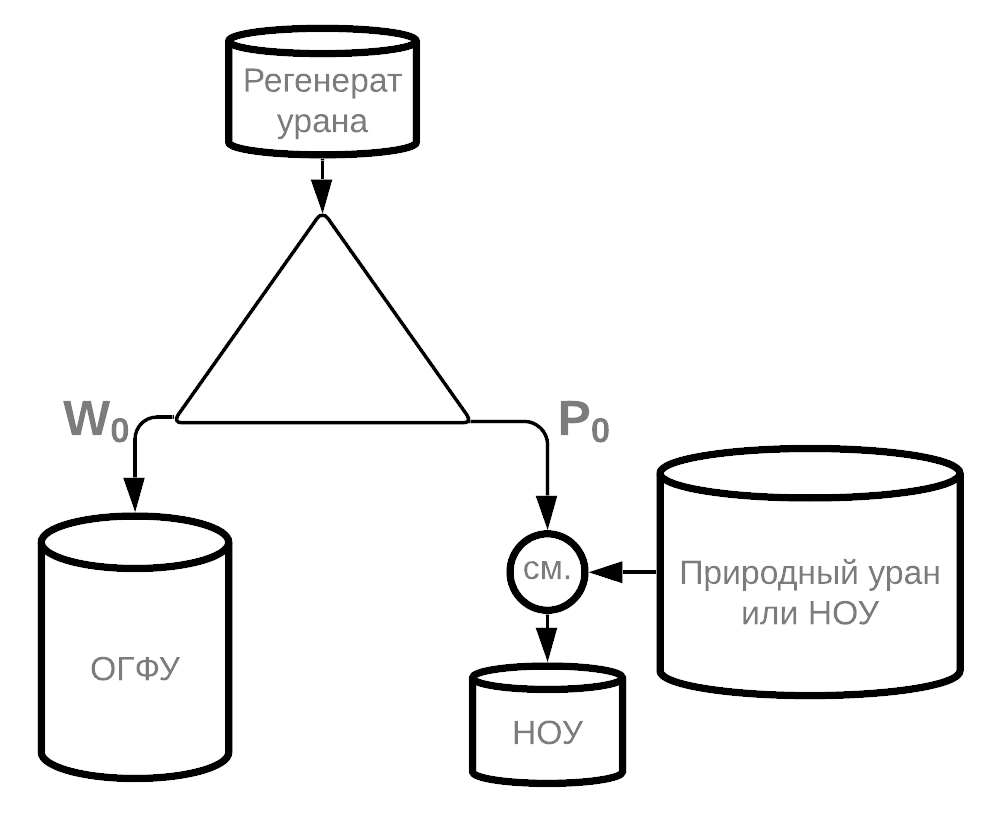
\includegraphics[scale=0.2]{cascades/ordinary/1}}
  \caption{Схема разбавления предварительно обогащенного регенерата природным ураном или низкообогащенным ураном. Обозначения: $P_0$ -- поток отбора легкой фракции каскада; $W_0$ -- поток отвального ОГФУ тяжелого конца каскада; $CM.$ -- узел смешения, на выходе из которого получается конечный продукт $НОУ$ -- низкообогащенный уран}\label{o1}
\end{figure}

Для получения обогащенного урана, удовлетворяющего всем требованиям, необходимо определить величину $C_{235, P_0}$ и отношение смешивания потоков $P_0$ и разбавителя. Указанные параметры определяли итерационно по следующей схеме. Сначала задавали начальное приближение для  $C_{235, P_0}$, после чего рассчитывали параметры каскада по описанной в предыдущем разделе процедуре. Далее, зная состав смеси урана в потоке $P_0$, определяли соотношение между потоками природного урана или обогащенного регенерата для получения финального продукта. При этом полученный в результате смешивания поток товарного НОУ должен отвечать ограничениям по концентрациям чётных изотопов, а отношение массы полученного НОУ к массе исходного регенерата должно соответствовать заданной величине. Это означает, что для успешного решения задачи одновременно должны быть выполнены условия на концентрации изотопов $^{232,234,235,236}$U и обеспечено заданное отношение между расходом регенерата и конечным продуктом. Однако при известной и заданной концентрации $^{235}$U в потоке разбавителя управляющих параметров в такой схеме только два: $C_{235, P_0}$ и отношение, в котором смешиваются обогащенный регенерат и разбавитель. Очевидно, что в этом случае не для любых исходных данных возможно подобрать требуемые параметры каскадной схемы.

Для иллюстрации сложности решения подобной задачи рассмотрим некоторые вспомогательные функции $\delta_1$ и $\delta_2$ (\ref{d1}).

\begin{equation}\label{d1} 
  \begin{cases}
    \delta_1=\left[C_{235,P\textit{экв.}}-\left(C_{235,P\textit{NU}}+KKP\times C_{236,P}\right)\right]\\
    \delta_2=\left[{(C_{232,P})}_{lim}-C_{232,P}\right]
  \end{cases}\
\end{equation}

По своему физическому смыслу величина $\delta_1$ представляет собой отклонение  $C_{235, P}$ -- концентрации изотопа $^{235}$U (выраженное в долях) в конечном продукте (после смешивания) -- от заданной величины, с учетом компенсации $^{236}$U. Величина $\delta_2$ представляет собой разность фактической концентрации $^{232}$U в окончательном продукте и требуемой величины в соответствии с принятым ограничением. Из таких определений очевидно, что в случае получения продукта, отвечающего необходимым условиям обе функции должны быть равны 0, причём при одних и тех же параметрах схемы. Фактически, функции $\delta_1$ и $\delta_2$ задают для рассматриваемой каскадной схемы систему уравнений, из которой можно найти её параметры при заданном отношении потоков регенерата и продукта.  Таким образом, для отклонений $\delta_1$ и $\delta_2$, система уравнений определяются следующим образом:


, где ККР -- коэффициент компенсации реактивности, $(C_{232,P})_{lim}$ -- величина предельно допустимой концентрации $^{232}$U в товарном НОУ (например, $5\cdot10^{-7}$\%).

Оговоримся, что, строго говоря, к этой системе надо добавить аналогичное условие (с невязкой $\delta_3$) на концентрацию $^{234}$U, однако, как будет показано ниже, даже в таком более простом варианте каскадная схема не может обеспечить одновременное выполнение всех требований, предъявляемых к составу конечного продукта.

В рамках работы были проведены вычислительные эксперименты, в которых варьировали $C_{235, P_0}$, а отношение потока $P_0$ к разбавителю из природного урана варьировали в диапазоне, где могут быть найдены допустимые решения. Для каждого случая пытались решить задачу обогащения регенерированного урана при описанных в разделе \ref{ch2_stat} внешних условиях задачи. Концентрацию $^{235}$U в потоке $W_0$ задавали равной 0,1\%. При расчёте параметров ординарного каскада во всех случаях предполагали, что в каскаде было реализовано условие несмешивания по относительной концентрации компонентов $^{235}UF_6$ и $^{238}UF_6$, так как эти два компонента имеются во всех используемых исходных смесях. Величину коэффициента разделения для компонентов  $^{235}UF_6$ к $^{238}UF_6$ приняли равной 1.2 \cite{smirnovEvolutionIsotopicComposition2012}. Все расчёты выполнены на примере регенерированного урана состава 1 (табл. \ref{is_compositions_2_5}).

Для удовлетворения заданным условиями задачи условиям, $\delta_1$ должна быть равна нулю (в численно решении относительная ошибка (отклонение от единицы отношений левой и правой частей равенства) не должна была превысить заданную для алгоритма величину $10^{-8}$), а $\delta_2$ должна принимать положительное значение, что будет соответствовать выполнению ограничения на предельное содержание $^{232}$U в НОУ-продукте.

На рис. \ref{delta1}--\ref{delta4} представлены зависимости величин $\delta_1$ и $\delta_2$ от соотношения смешиваемых потоков (в диапазоне от 1 до 20, в который попадают все значимые для иллюстрации области значений величин $\delta_1$ и $\delta_2$), взятых для различных значений $C_{235, P_0}$ (рис. \ref{delta1}--\ref{delta4}). Значения $C_{235, P_0}$ на рис. \ref{delta1}--\ref{delta4} представлены в диапазоне от 7 до 50\% в иллюстративных целях,  также как и соотношения смешиваемых потоков, так как эти диапазоны достаточны, чтобы продемонстрировать невозможность одновременного удовлетворения условия компенсации $^{236}$U и выполнения заданного ограничения по $^{232}$U в получаемом товарном НОУ. Чтобы сопоставить указанные величины на одном рисунке, величина $\delta_2$ была взята с поправкой (умножена на специально подобранный числовой коэффициент, который равен $10^{6}$).

Как видно из рисунков \ref{delta1}-\ref{delta4} функции $\delta_1$ и $\delta_2$ принимают удовлетворяющие заданным условиям задачи значения при различных значениях аргумента. Таким образом, полученные результаты показывают невозможность одновременного удовлетворения условия компенсации $^{236}$U и выполнения заданного ограничения по $^{232}$U в получаемом товарном НОУ. По крайней мере это справедливо для рассмотренного изотопного состава. Дополнительные расчёты для состава №2 рецикла подтвердили те же выводы. Следовательно, данную схему нельзя рассматривать в качестве способа обогащения регенерированного урана в условиях его многократного рецикла.


\begin{figure}[ht]
  \begin{minipage}{.5\textwidth}
    \centering
    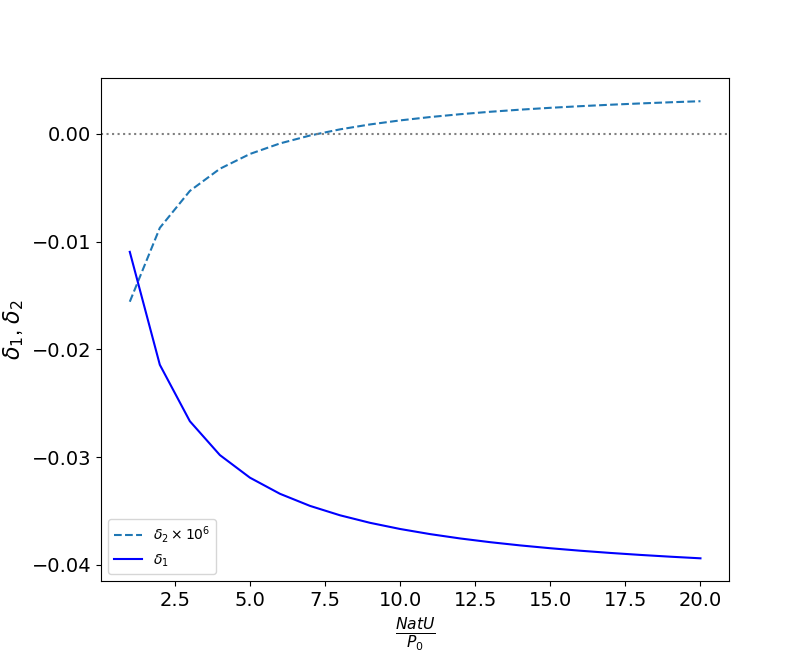
\includegraphics[width=.8\linewidth]{images/plots/7}  
    \caption{Концентрация $^{235}$U в предварительно обогащенном регенерата равна 7\%}
    \label{delta1}
  \end{minipage}
  \begin{minipage}{.5\textwidth}
    \centering
    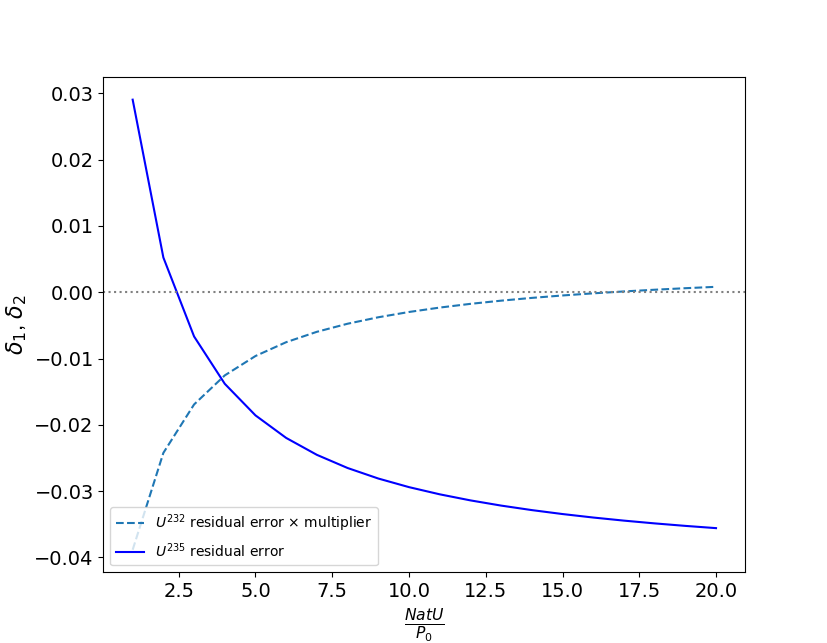
\includegraphics[width=.8\linewidth]{images/plots/15}  
    \caption{Концентрация $^{235}$U в предварительно обогащенном регенерата равна 15\%}
    \label{delta2}
  \end{minipage}
  \begin{minipage}{.5\textwidth}
    \centering
    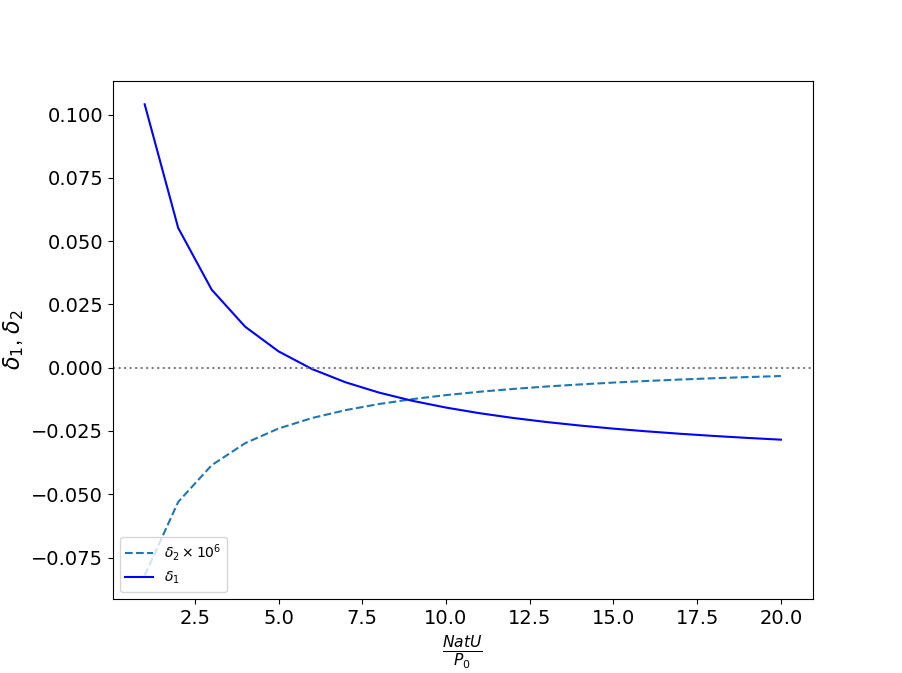
\includegraphics[width=.8\linewidth]{images/plots/30}  
    \caption{Концентрация $^{235}$U в предварительно обогащенном регенерата равна 30\%}
    \label{delta3}
  \end{minipage}
  \begin{minipage}{.5\textwidth}
    \centering
    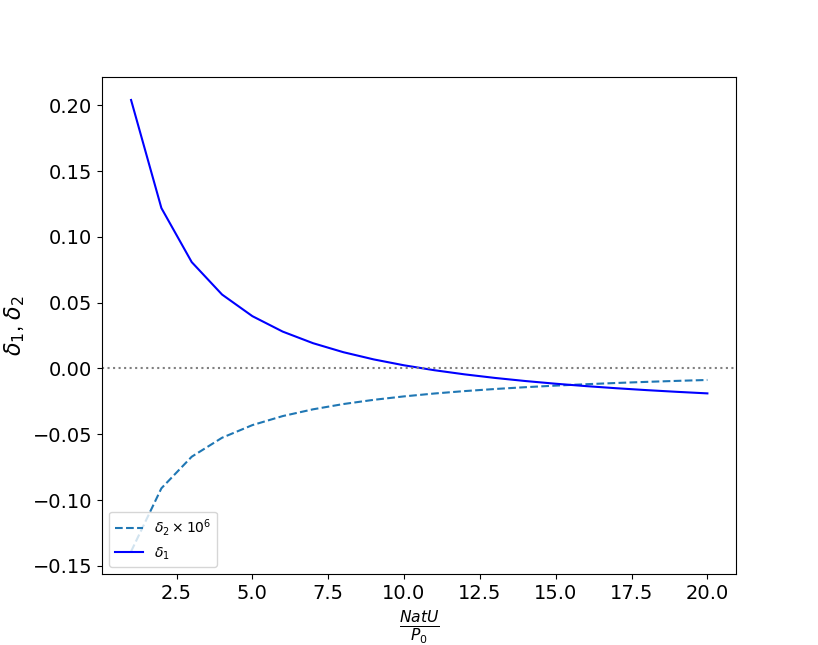
\includegraphics[width=.8\linewidth]{images/plots/50}  
    \caption{Концентрация $^{235}$U в предварительно обогащенном регенерата равна 50\%}
    \label{delta4}
  \end{minipage}
 \end{figure}


\subsection{Схема с разбавлением предварительно обогащенного регенерата низкообогащенным ураном}

Если в схеме, рассмотренной выше (рис. \ref{o1}), заменить разбавитель предварительно обогащенного регенерата (рис. \ref{o1}) с природного урана на низкообогащенный уран, не содержащий четных изотопов (например, изготовленный из природного урана), для данного состава можно найти решение, когда одновременно выполнены условия равенства нулю обеих невязок ($\delta_1$ и $\delta_2$). Данная схема может быть рассмотрена в качестве модификации варианта, описанного в предыдущем разделе. Нахождение решения для такой схемы обусловлено появлением дополнительного управляющего параметра -- концентрации $^{235}$U в потоке НОУ-разбавителя.  Несмотря на это, в подобном варианте каскадной схемы может быть не выполнено условие максимального использования регенерированного урана, состоящее в равенстве отношения потоков исходного регенерата и товарного НОУ заданной величине.

Чтобы оценить возможность решения задачи с использованием каскадной схемы с разбавлением предварительно обогащенного регенерата низкообогащенным ураном (рис. \ref{o1}), проведены вычислительные эксперименты, в рамках которых варьировались следующие параметры схемы:
\begin{enumerate}
  \item концентрация $^{235}$U в потоке $P_0$
  \item концентрация $^{235}$U в потоке $W_0$
\end{enumerate}

Варьирование этих параметров позволяет регулировать относительные концентрации компонентов в смеси, в частности, пары изотопов $^{232}$U и $^{235}$U. Это позволяет обеспечивать получение различных вариантов изотопного состава конечного продукта. 

\begin{figure}[ht]
  \centerfloat{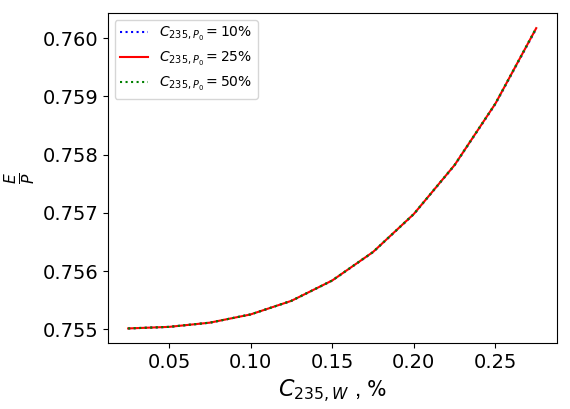
\includegraphics[scale=0.5]{images/plots/3_6}}
  \caption{Расход регенерата на единицу конечного НОУ-продукта для различных  $C_{235, P}$ и $C_{235, W}$ каскада, обогащающего регенерат (кривые совпадают)}\label{Figure_10}
\end{figure}

\begin{figure}[ht]
  \centerfloat{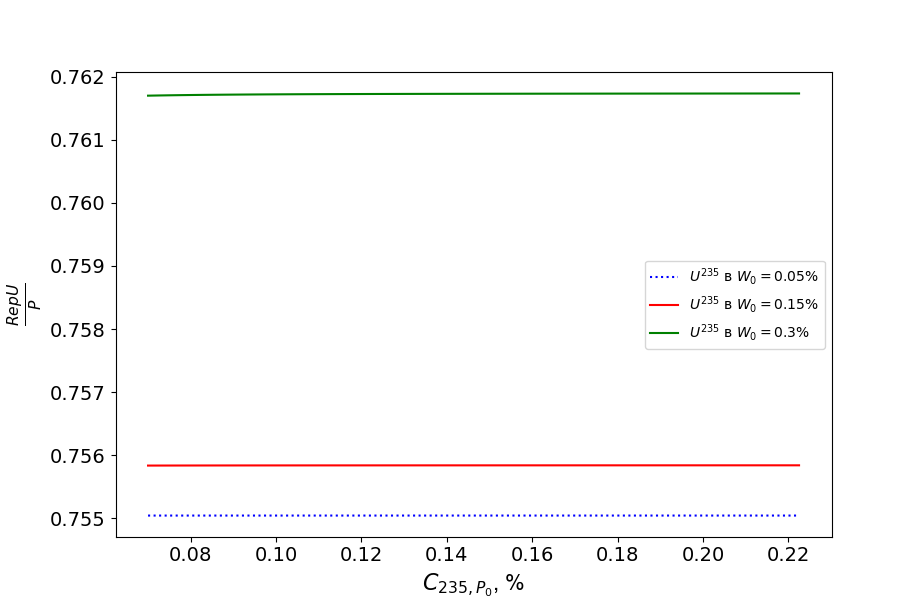
\includegraphics[scale=0.5]{images/plots/3_61}}
  \caption{Расход регенерата на единицу конечного НОУ-продукта для различных $C_{235, P}$ и $C_{235, W}$ каскада, обогащающего регенерат}\label{Figure_10_1}
\end{figure}

\begin{figure}[ht]
  \centerfloat{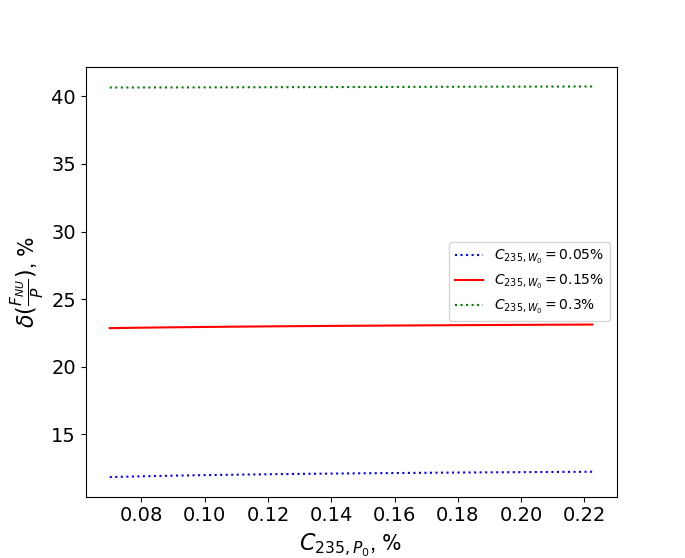
\includegraphics[scale=0.5]{images/plots/3_7}}
  \caption{Экономия природного урана на единицу НОУ-продукта  для различных $C_{235, P}$ и $C_{235, W}$ каскада, обогащающего регенерат}\label{fig:sc2_2}
\end{figure}

На рис. \ref{Figure_10}-\ref{fig:sc2_2} представлены зависимости отношения потоков исходного регенерата и конечного продукта, а также такие ключевые характеристики схемы как экономия природного урана и экономия работы разделения, получаемые при обогащении регенерированного урана в рассматриваемой каскадной схеме. 
Анализ кривых рисунков \ref{Figure_10}-\ref{Figure_10_1}, отражающих зависимости расхода регенерата на единицу НОУ-продукта ($\frac{NatU}{P_{0}}$) от $C_{235, W_0}$ при трёх различных концентрациях данного изотопа в потоке $P_0$ (или от концентрации $^{235}$U в потоке $P_0$ при различных концентрациях $^{235}$U в $W_0$, показывает невозможность выполнить условия возврата заданной доли регенерата на единицу продукта в такой каскадной схеме ($C_{235, P_0}$, $C_{235, W_0}$) в доступном диапазоне варьирования её свободных параметров. Причем отношение используемого регенерата к НОУ-продукту меняется лишь незначительно с изменением $C_{235, W_0}$, и константно при разных концентрациях $C_{235, P_0}$. Последнее означает, что изменение данного параметра может оказывать влияние на величину затрат работы разделения или расхода природного урана (см. рисунки \ref{fig:sc2_2}, \ref{Figure_13}), но не долю возвращаемого в воспроизводство топлива регенерата.
Как следует из анализа рисунка \ref{fig:sc2_2}, варьирование концентраций $^{235}$U в потоках $P_0$ и $W_0$ позволяет варьировать экономию природного урана, обеспечив расход на уровне $\approx$6,5-6,7 кг на 1 кг конечного НОУ-продукта для всего исследуемого диапазона параметров. Это означает, что при заданном интервале параметров, рассматриваемая схема обеспечивает экономию природного урана на уровне 15--40\%, по сравнению со схемой получения НОУ только из природного сырья при таких же значениях концентрации $^{235}$U в $W_0$ соответственно.
% , для которого удельный расход природного урана составляет $\approx$7,93 (см. Приложение).

В качестве дополнительной иллюстрации полученных данных на рис.\ref{Figure_13} представлены зависимости экономии работы разделения (по сравнению со схемой прямого обогащения природного урана) от величины $C_{235, W_0}$ при различных концентрациях данного изотопов в потоке $P_0$. Область отрицательных значений потерь работы разделения на рис. \ref{Figure_13} соответствует ее экономии. Как следует из изучения характера кривых, уменьшение $C_{235, W_0}$ позволяет увеличить экономию работы разделения за счет более эффективного извлечения $^{235}$U из регенерата. Слияние кривых, соответствующих различным концентрациям $^{235}$U в обогащенном регенерате, обусловлено эквивалентностью масс $^{235}$U в каждом из этих потоков, что отражает постоянство вклада обогащенного регенерата в формирование конечного продукта.

% \begin{figure}[ht]
%   \centerfloat{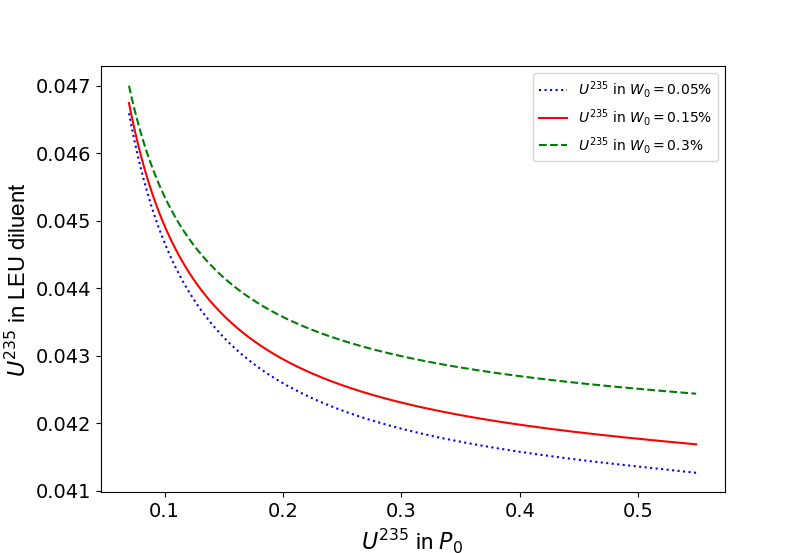
\includegraphics[scale=0.5]{images/plots/sc2_LEU_D}}
%   \caption{Концентрация $^{235}$U в разбавителе, необходимая для получения свежего НОУ для различных концентраций $^{235}$U в потоках продукта и отвала каскада, обогащающего регенерат}\label{fig:sc2_LEU_D}
% \end{figure}


\begin{figure}[ht]
  \centerfloat{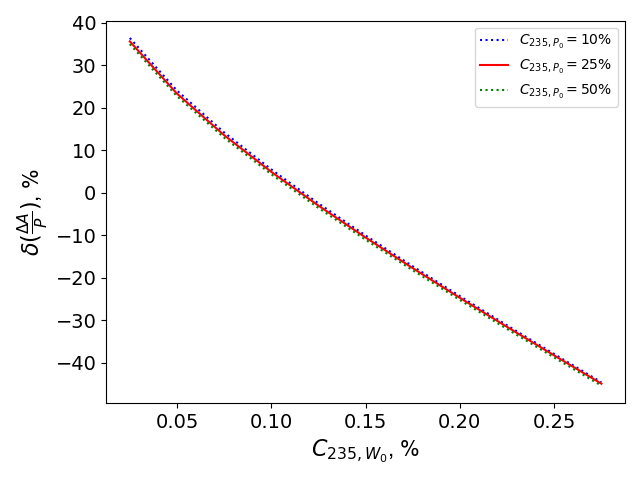
\includegraphics[scale=0.5]{images/plots/3_8}}
  \caption{Экономия работы разделения по отношению к ординарному каскаду для обогащения природного урана для различных концентраций $^{235}$U в потоках продукта и отвала каскада, обогащающего регенерат}\label{Figure_13}
\end{figure}


% Проиллюстрировать затраты на работу разделения от составных  частей каскадной схемы, можно с помощью рис.\ref{myplot}, который показывает, что доля центрифуг для приготовления разбавителя из природного урана выше, чем доля центрифуг, задействованных для предварительного обогащения регенерата, и эта пропорция уменьшается с понижением содержания $^{235}$U в $W_0$.

% \begin{figure}[ht]
%   \centerfloat{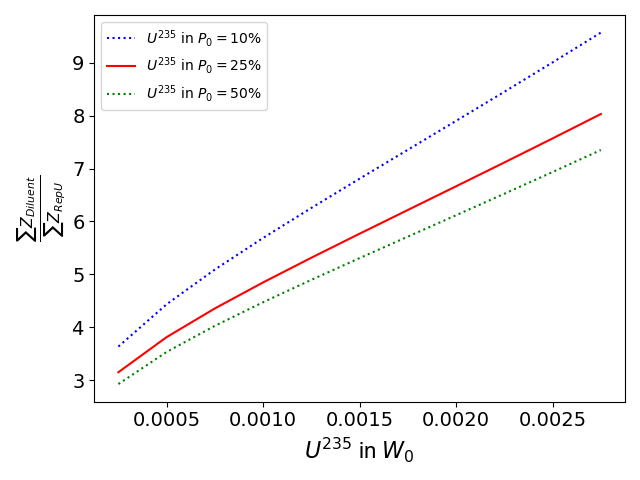
\includegraphics[scale=0.5]{images/plots/myplot}}
%   \caption{Отношение количества центрифуг в каскаде, производящем разбавитель из природного урана, к количеству центрифуг, задействованных для предварительного обогащения регенерата, для различных концентраций $^{235}$U в потоках продукта и отвала каскада, обогащающего регенерат}\label{myplot}
% \end{figure}

Подытоживая анализ результатов вычислительных экспериментов для данной модификации ординарного каскада для обогащения регенерированного урана, можно заключить, что она непригодна для решения задачи обогащения в условиях многократного рецикла, так как с помощью нее нет возможности использовать весь регенерированный уран на производство НОУ-продукта, как показано на рис. \ref{Figure_10}. Однако, такую схему можно использовать для решения задачи повторного использования урана для возврата (дообогащения) регенерата с относительно низким исходным содержанием чётных изотопов, например, в случае обогащения регенерата первого рецикла.


\subsection{Анализ схемы с разбавлением предварительно обогащенного природного урана регенератом}

Проанализируем возможность решения задачи обогащения регенерированного урана со всеми ограничениями в каскадной схеме с разбавлением предварительно обогащенного природного урана регенератом (рис. \ref{o2}). Принцип работы такой схемы состоит в том, что предварительно обогащенный природный уран смешивается с возвращаемым в топливный цикл регенерированным ураном. Уровень предварительного обогащения (перед смешением) природного урана и отношение потоков обогащенного природного урана к регенерату определяются исходя из условий задачи. Таким образом, данная схема в принципе аналогична схеме с разбавлением предварительно обогащенного регенерата природным ураном (рис. \ref{o1}). Это означает, что ей присущи те же недостатки, что и упомянутой схеме, а именно: в ней число управляющих параметров меньше, чем число условий, предъявляемых к конечному продукту. 

\begin{figure}[ht]
  \centerfloat{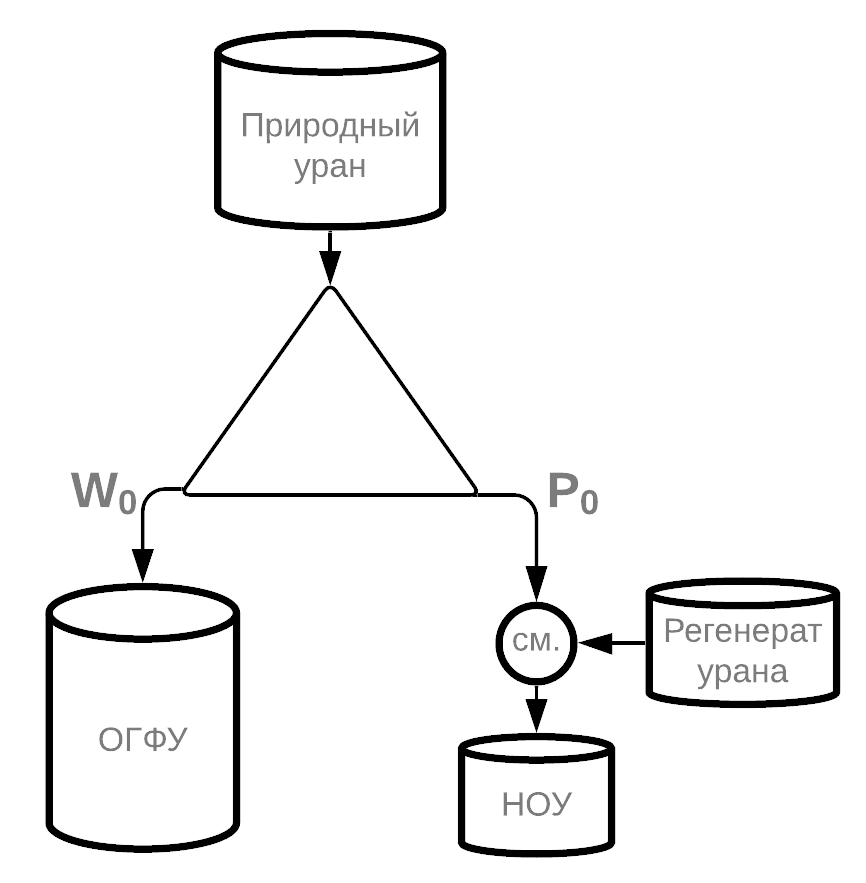
\includegraphics[scale=0.2]{cascades/ordinary/2}}
  \caption{Схема каскада с разбавлением предварительно обогащенного природного урана регенератом. Обозначения: $P_0$ -- поток отбора легкой фракции каскада; $W_0$ -- поток отвального ОГФУ тяжелого <<конца>> каскада; $CM.$ -- узел смешения, на выходе из которого получается конечный НОУ-продукт $НОУ$  -- низкообогащенный уран}\label{o2}
\end{figure}

Для ответа на вопрос о возможности использования данной схемы для обогащения регенерата в условиях многократного рецикла были проведены вычислительные эксперименты, в рамках которых варьировали величину концентрации $^{235}$U в обогащенном природном уране и отношение, в котором смешиваются разбавитель с регенератом с целью найти такой набор параметров схемы, при которых сформулированная в разделе \ref{ch2_stat} задача будет решена. Как и в рассмотренных выше примерах моделирование процесса обогащения урана в каскаде осуществляли с использованием R-каскада. Концентрацию $^{235}$U в отвале каскада задавали равной 0,1\%.

Из результатов вычислительных экспериментов следует, что для рассматриваемой схемы возможно получение решения, удовлетворяющего заданным ограничениям на концентрации изотопов $^{232,234,236}$U. Однако, как и в случае применения схемы рис. \ref{o1}, одновременно с этими условиями не удаётся удовлетворить условие возврата заданной массы регенерата. В результате вместо заданной величины отношения массы исходного регенерата к продукту -- 0,93, фактические значения не превысили величины 0,755. Данные результаты свидетельствуют о том, что такая схема обогащения регенерата не решает поставленную задачу для произвольного изотопного состава регенерата и, следовательно, не может быть применена в условиях многократного рецикла урана в топливе легководных реакторов.

\subsection{Анализ схемы с разбавлением регенерата природным ураном перед подачей в ординарный трехпоточный каскад}

Еще одним вариантом каскадной схемы для обогащения регенерированного урана, основанной на использовании ординарного каскада является схема, в которой смешивание и разбавление регенерата происходит непосредственно перед подачей в каскада для последующего обогащения (рис. \ref{o3}). В качестве разбавителя здесь, как правило, рассматривают природный уран. Соотношение, в котором следует смешать природный и регенерированный уран определяют, исходя из ограничений на четные изотопы в конечном НОУ-продукте.

\begin{figure}[ht]
  \centerfloat{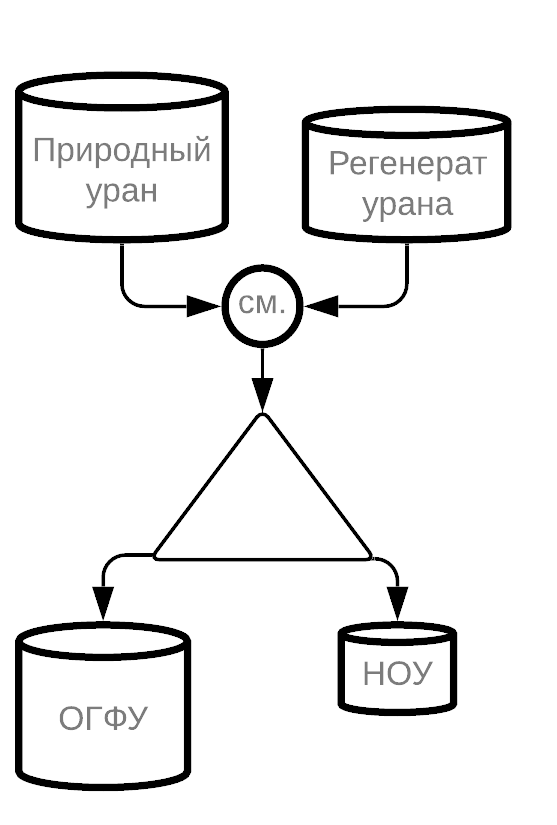
\includegraphics[scale=0.25]{cascades/ordinary/3}}
  \caption{Схема каскада со смешением регенерата и природного урана перед подачей на питание ординарного каскада. Обозначения: см. -- смесь входящих сырьевых потоков, образующих питание каскада; $НОУ$ -- конечный НОУ-продукт схемы}\label{o3}
\end{figure}

В случае, если разбавитель известен, то для такой схемы существует единственный управляющий параметр -- это отношение, в котором смешиваются потоки регенерата и природного урана. Очевидно, что с ростом доли регенерата в совокупном питании каскада будут возрастать концентрации чётных изотопов в потоке отбора каскада. Это обуславливает тот факт, что существует некоторое критическое значение этого отношения, начиная с которого уже невозможно будет соблюсти, как минимум, ограничение на концентрацию изотопа $^{232}$U. Для рассматриваемой схемы также были проведены вычислительные эксперименты, в которых варьировали отношение разбавления между регенератом и разбавителем, в качестве которого рассматривали уран природного состава. Как и во всех рассмотренных в рамках данной главы примерах исходные условия соответствовали задачи, описанной в разделе \ref{ch2_stat}, а в качестве расчётной модели использован R-каскад. Расчёты проведены на примере состава 1 таблицы \ref{is_compositions_2_5}. 

На рис. \ref{sc3_1.second} отражена взаимосвязь доли регенерата в питании каскада, концентрации $^{232}$U в конечном продукте и отношения потока исходного регенерата к потоку продукта. Кривые построены при различных $C_{235, W}$. Как следует из анализа представленных зависимостей, во всех случаях величина концентрации  $^{232}$U достигает предельного значения ($5\cdot10^{-7}$\%) ранее, чем отношение между исходным регенератом и продуктом достигнет требуемого значения -- 0,93. Это означает, что и эта схема также не позволяет решить полностью задачу обогащения регенерата с относительно высоким содержанием чётных изотопов, не позволяя расходовать заданное количество регенерата на единицу конечного НОУ-продукта. 

% \begin{figure}[ht]
%   \centerfloat{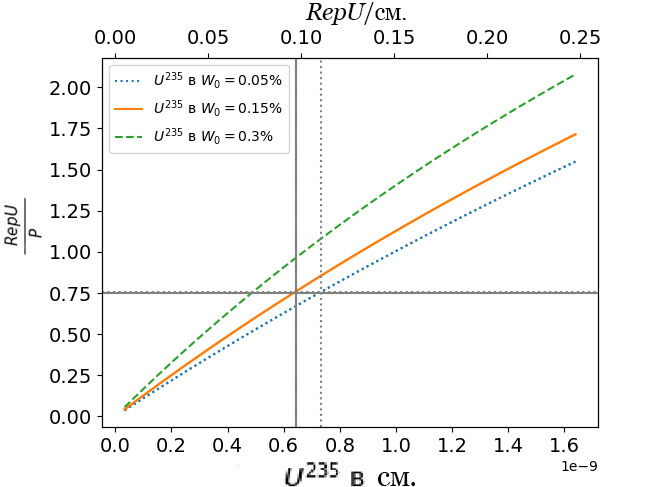
\includegraphics[scale=0.5]{images/plots/3.11new}}
%   \caption{Расход регенерированного урана на единицу НОУ-продукта  при различной концентрации $^{232}$U в питающем потоке каскада для различных концентраций $^{235}$U в потоке отвала. Обозначения: см. - смесь природного урана и регенерата, подаваемая на питание каскада}\label{sc3_1.second}
% \end{figure}

\begin{figure}[ht]
  \centerfloat{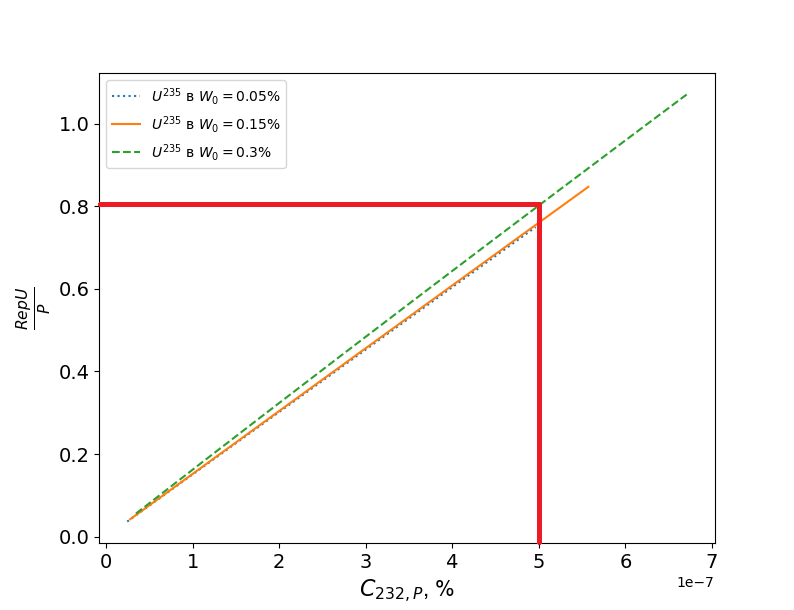
\includegraphics[scale=0.5]{images/plots/3_11}}
  \caption{Расход регенерированного урана на единицу НОУ-продукта  при различной концентрации $^{232}$U в питающем потоке каскада для различных концентраций $^{232}$U в потоке НОУ-продукта}\label{sc3_1.second}
\end{figure}


\subsection{Общий вывод для схем возврата регенерата в ЯТЦ на основе ординарного каскада}

Описанные выше результаты вычислительных экспериментов, проведенных для анализа применимости схем на основе простейших модификаций ординарного каскада для решения сформулированной в главе \ref{ch1} задачи обогащения регенерированного урана, показали что такие схемы не могут решить подобную задачу в условиях  многократного рецикла. Это обусловлено ухудшением изотопного состава урана по мере прохождения им серии топливных циклов, что выражается в накоплении $^{232}$U и других чётных изотопов. При этом исходная концентрация $^{232}$U питающей смеси, начиная со второго рецикла, превышает уровень допустимый в конечном продукте, поэтому схемы, основанные на ординарном каскаде, которые только разбавляют этот изотоп, не эффективны для решения поставленной задачи. Тем не менее, если рассматривать подобные схемы для обогащения регенерированного урана, прошедшего только однократное облучение или допустить <<послабление>> ограничений на концентрации чётных изотопов, то подобные схемы, безусловно, могут быть применены для решения задачи обогащения регенерированного урана.

При этом закономерно возникает следующий вопрос: возможно ли априорно оценить возможность решить поставленную выше (\ref{ch2_stat}) задачу в таких модификациях ординарного каскада? 

На этот вопрос можно ответить, обратившись к уравнениям баланса компонентов в каскаде \ref{GrindEQ__1_21_} по крайней мере в случае вариантов каскадных схем, где регенерированный уран поступает в каскад для обогащения. Если записать уравнение \ref{GrindEQ__1_21_} для изотопа $^{232}$U и, учитывая, его малую концентрации в исходной смеси сделать предположение о том, что его концентрация в отвале каскада будет стремиться к нулю. Данное предположение может быть вполне оправдано, если отвальная часть каскада имеет достаточное число ступеней. В этом случае $^{232}$U, являясь самым лёгким в смеси регенерированного урана, будет активнее остальных компонентов концентрироваться в отборе каскада. Это означает, что для изотопа $^{232}$U уравнение \ref{GrindEQ__1_21_} можно переписать в следующем виде, пренебрегая слагаемым с потоком отвала каскада:

\begin{equation} \label{GrindEQ__1_21__} 
  \begin{array}{l} {\quad \quad \quad \quad \quad  E+F=P+W,} \\ {FC_{i,F} + EC_{i,E} =PC_{i,P} +WC_{i,W} ,\;  i=1,2,...,m.} \end{array} 
\end{equation} 

% \begin{equation}
% \label{eq_232_balance}
%   C_{232,P} \approx \frac{RepU}{P} C_{232,RepU}
% \end{equation}

\begin{equation}
  \label{eq_232_balance_}
    C_{232,P} \approx \frac{E}{P} C_{232,E}
  \end{equation}

Величина $\frac{E}{P}$ в приведенном выше уравнении и является отношением (исходный регенерат)/продукт. Если учесть, что типичные значения этого отношения составляют величину $\approx$0,9-0,95, то станет очевидно, что это условие будет выполнено только, если концентрация $^{232}$U в исходном регенерате ниже, чем ограничение на $^{232}$U в конечном продукте. 
С помощью уравнения \ref{eq_232_balance} можно вычислить максимально возможную долю питающего потока, содержащего $^{232}$U, как неизвестную переменную уравнения \ref{eq_232_balance}. Например, для состава 1 таблицы \ref{is_compositions_2_5}, который был использован в рассмотренных выше примерах получаем:

% \begin{equation}
%   \label{eq_232_balance_X}
%     5 \times 10^{-7} \% \approx X \times 6.622 \times 10^{-7} \% \Rightarrow X \approx 0.755
% \end{equation}

% \begin{equation}
%   \label{eq_232_balance_X}
%     \frac{RepU}{P} \leq 0,755
% \end{equation}

\begin{equation}
  \label{eq_232_balance_X_}
    \frac{E}{P} \leq 0,755
\end{equation}

% \begin{equation}
%   \label{eq_232_balance_X_}
%     \frac{E}{P} \leq 0,5
% \end{equation}

Снова анализируя представленные в предыдущих разделах данные, легко увидеть, что полученные в результате прямого численного расчёта предельные величины отношений (исходный регенерат)/продукт приблизительно и составляют такую величину.
Подобный подход позволяет аналитически оценить возможность применения схем на основе простейших модификаций ординарного каскада, исходя из изотопного состава регенерата. Следует отметить также, что подобные оценки можно также применять и для каскадных схем, в которых регенерат разбавляют уже внутри каскада, путём его подачи в качестве дополнительного питания, поскольку такие схемы по сути являются также только разбавляющими.

\section{Обоснование необходимости составных схем}\label{sec:ch2/sec2}

Как следует из предыдущей части настоящей главы, на текущий момент в принципе имеются способы, позволяющие обеспечить выполнение требований по четным изотопам урана при обогащении регенерата. Однако основной проблемой, решаемой в рамках настоящей диссертационной работы, является поиск варианта каскадной схемы, позволяющей одновременно выполнить ограничения по концентрациям четных изотопов и задействовать в обогащении весь имеющийся регенерат в условиях неопределенности его изотопного состава при многократном рецикле.

Если анализировать причины невозможности возврата массы регенерата в производство топлива в многочисленных модификациях каскада для обогащения многократно облученного регенерата, то становится очевидным, что это, во многом, связано с нарастанием относительных концентраций <<легких>> изотопов (в первую очередь $^{232}$U) и $^{235}$U, а поскольку данные изотопы концентрируются вместе на легком <<конце>> каскада, то единственным способом понизить отношение их концентраций -- это разбавить материалом, не содержащим $^{232}$U, например на входе в каскад. Как показали результаты, описанных в этой главе вычислительных экспериментов, для составов с достаточно высоким исходным содержанием $^{232}$U невозможно подобрать такой разбавитель, чтобы удовлетворить одновременно и условие полного возврата массы регенерата в цикл и условия на содержание четных изотопов.

Из приведенного выше анализа следует, что эффективная каскадная схема для обогащения регенерата урана при многократном рецикле должна обеспечивать не только разбавление регенерата, но и хотя бы частичную его очистку от чётных изотопов. Поэтому возможные варианты решения задачи, по-видимому, должны быть основаны на использовании схем двойных каскадов, в том числе, описанных в Главе \ref{ch1}. В связи с этим интерес ответ на вопрос о возможности прямого обогащения регенерата с повышенным содержанием чётных изотопов в двойном каскаде с целью решения задачи обогащения регенерата в наиболее общей постановке. Этот вопрос и рассмотрен в следующих разделах настоящей главы.



\section{Двойной каскад}\label{sec:ch2/dvoynoy}

Возможностью осуществить решение является двойной каскад, представленный в обзоре Гл. \ref{ch1/dvoynoy}, представляющий собой последовательное соединение двух каскадов (рис. \ref{fig:double_ru}). 

\begin{figure}[ht]
  \centerfloat{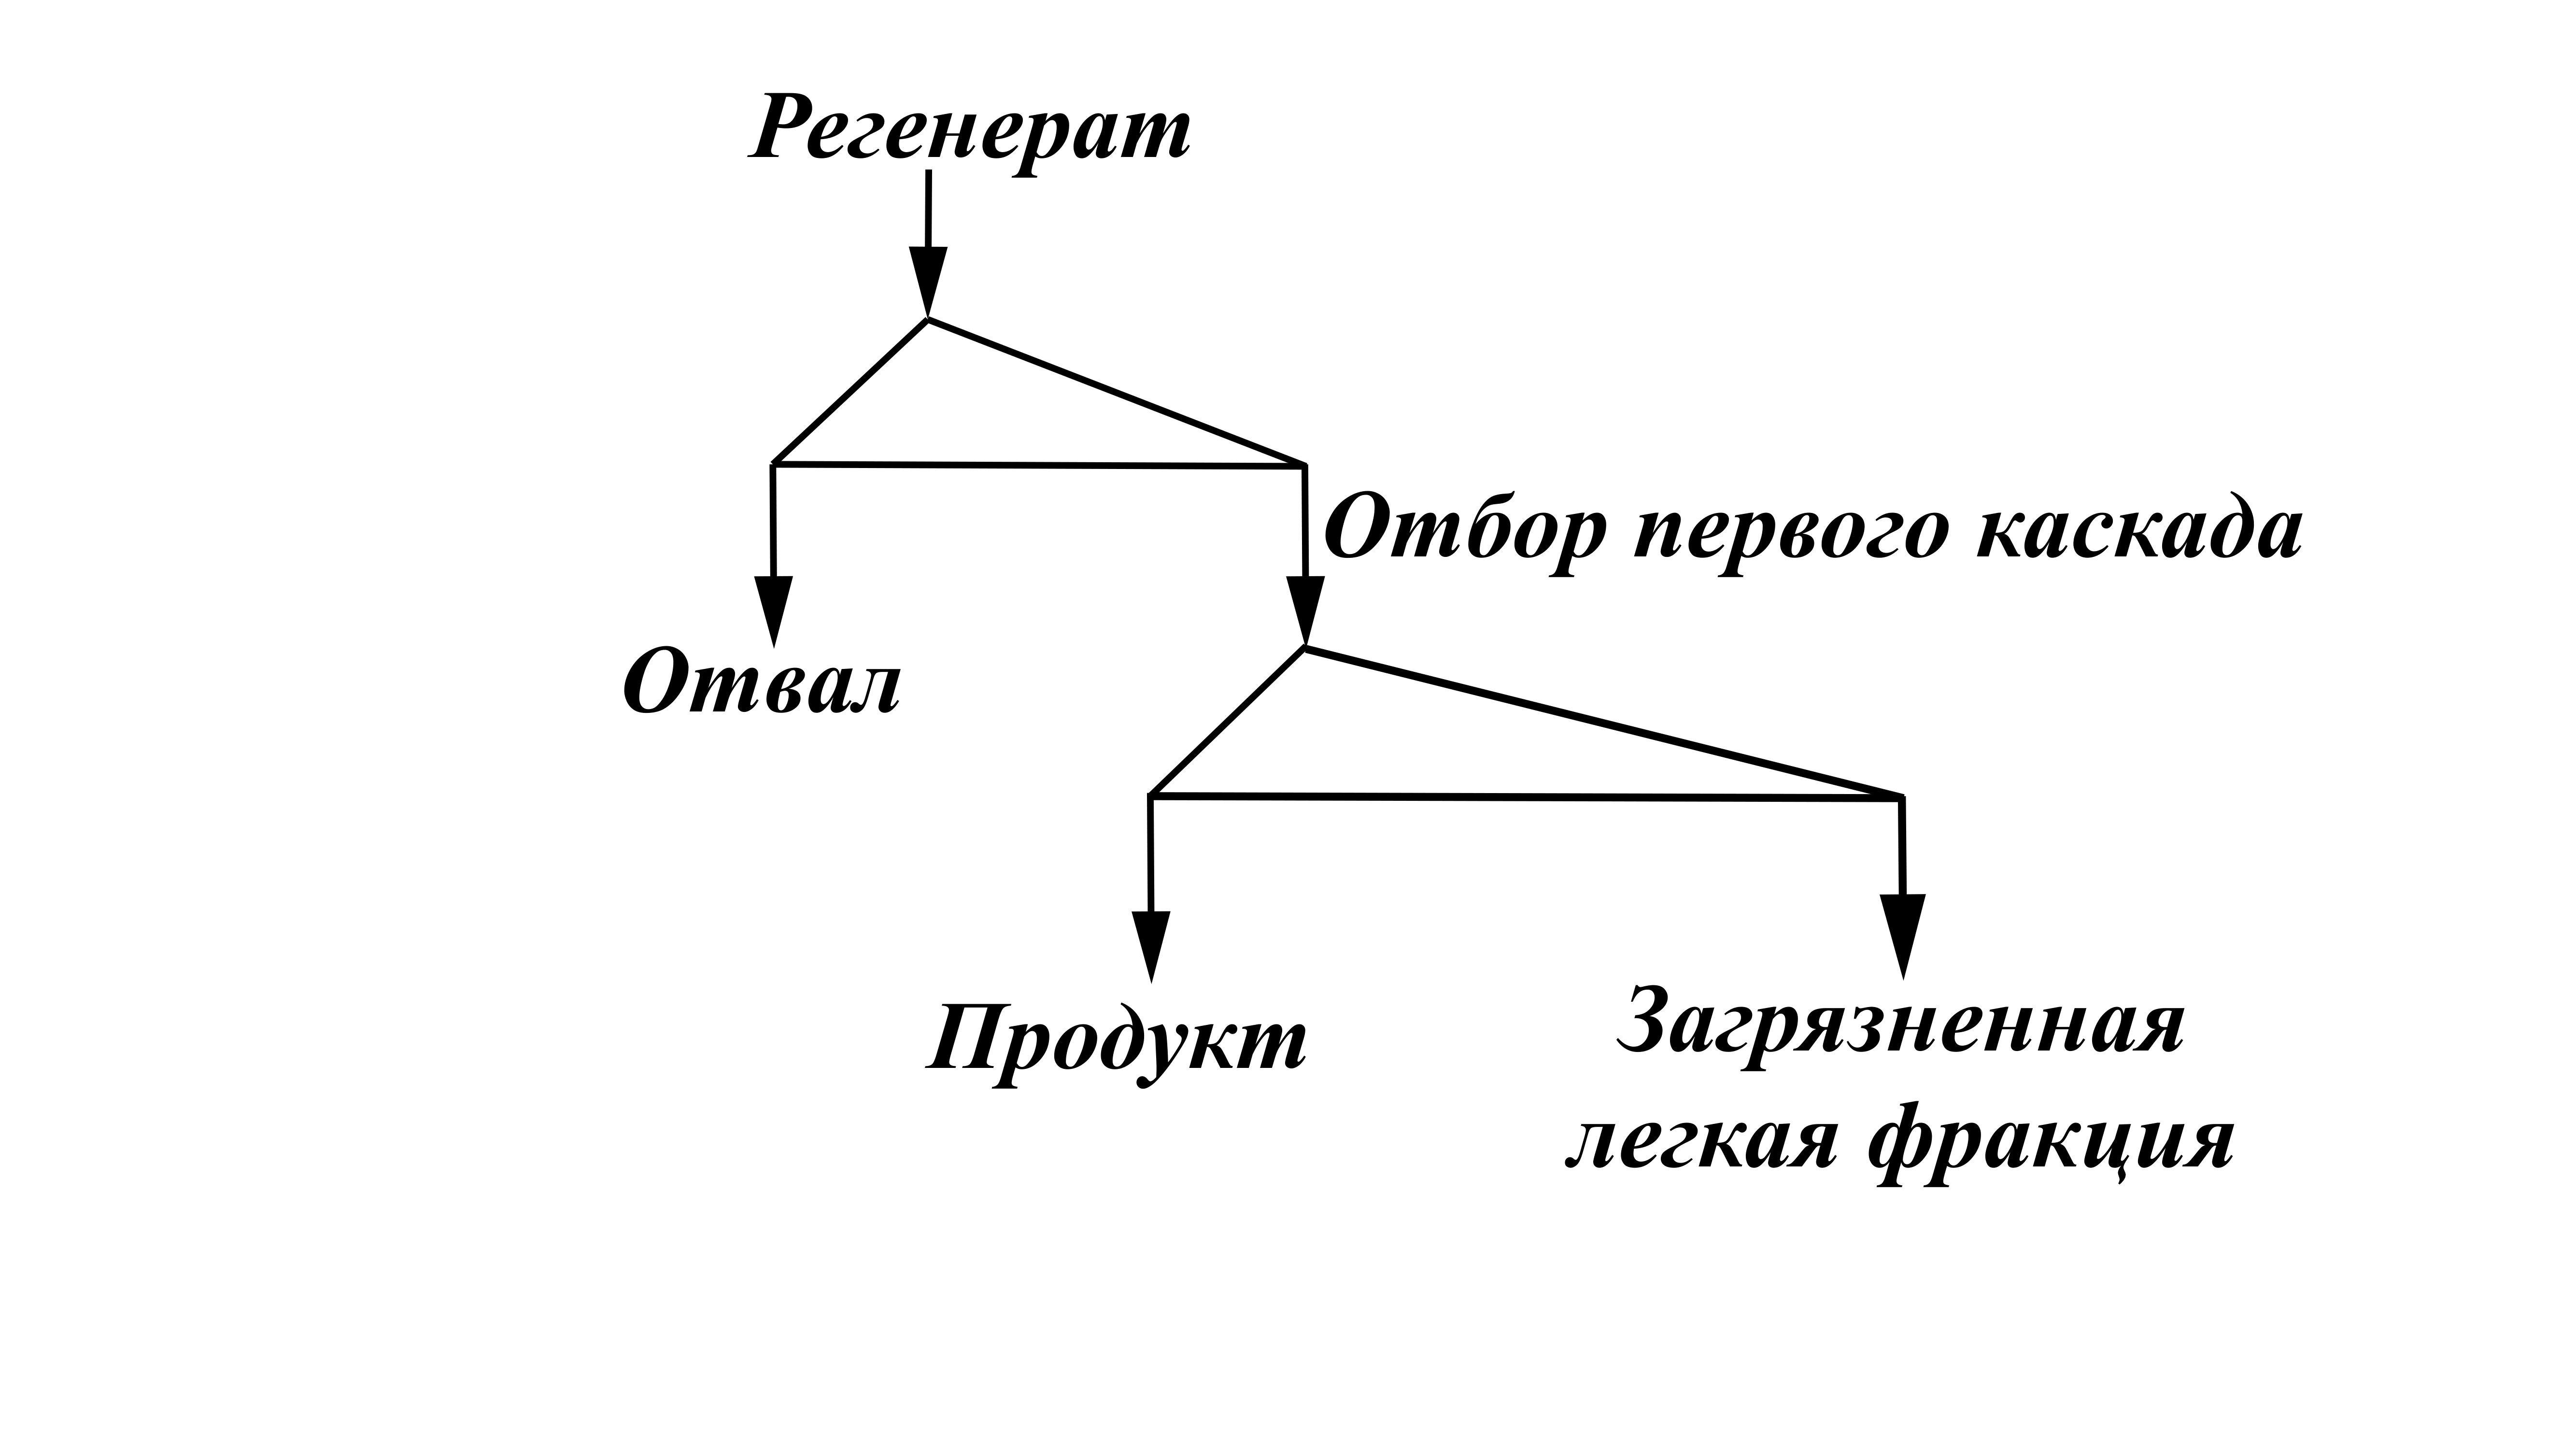
\includegraphics[scale=0.07]{cascades/double_ru}}
  \caption{Двойной каскад}\label{fig:double_ru}
\end{figure}

Анализируя уравнения, описывающие модель двойного <<квазиидеального>> каскада, а также учитывая сформулированную выше постановку задачи, получаем 3 неизвестных переменные: 1) $C_{235, P_1}$; 2) $C_{235, P_2}$; 3) $C_{235, W_2}$; и два независимых уравнения, характеризующих целевую систему:

\begin{enumerate}
    \item $\delta_{1}=C_{235,P\textit{ экв.}}-(C_{235,P\textit{ NU}}+\Delta C_{235})$ -- невязка по концентрации $^{235}$U в конечном НОУ-продукте, с учетом поправки на присутствие изотопа $^{236}$U. Величина $\delta_{1}$ фактически определяет точность достижения условия компенсации $^{236}$U;
    \item $\delta_{2}=C_{232,P\textit{ расч.}}-C_{232,P\textit{ треб.}}$ -- разница между рассчитанным значением концентрации $^{232}$U в конечном НОУ-продукте и заданным ограничением для концентрации этого изотопа.
\end{enumerate}

Таким образом, для нахождения 3-х переменных, имея 2 уравнения, получаем 1 свободную переменную, которую следует рассматривать в в качестве оптимизационной. В качестве такой переменной была выбрана $C_{235, P_2}$, которая затем была подобрана в ходе оптимизационной процедуры на критерий затрат работы разделения. Отметим также, что дополнительно для нахождения оптимального распределения потока по ступеням (для подбора формы каскада, соответствующей наименьшему суммарному потоку) было осуществлено варьирование величин $g_{i}$, которое было организовано перебором возможных опорных компонент $M_{k1}$ и $M_{k2}$ для ординарных каскадов 1 и 2, входящих в схему.


В качестве ключевых оцениваемых характеристик будем опираться на те же интегральные характеристики, отражающие экономику разделительного процесса, что использовались для анализа схем на основе ординарного каскада:
\begin{enumerate}
    \item $\delta(\frac{\Delta A}{P})$ -- экономия работы разделения относительно референтной схемы трехпоточного каскада для обогащения природного урана (см. Приложение). Наибольшая экономия соответствует минимуму суммарного потока схемы \ref{GrindEQ__1_73_}. Если величина отрицательная, абсолютное значение соответствует потерям работы разделения, по сравнению с референтной схемы трехпоточного каскада для обогащения природного урана;
    \item $\delta(\frac{F_{NU}}{P})$ -- экономия природного урана относительно референтной схемы трехпоточного каскада для обогащения природного урана.  Наибольшая экономия соответствует минимуму удельного расхода природного урана схемы. Если величина отрицательна, абсолютное значение соответствует перерасходу природного урана, по сравнению с референтной схемы трехпоточного каскада для обогащения природного урана.
\end{enumerate}

Ниже приведены результаты анализа применимости схемы двойного каскада для возврата регенерата в ЯТЦ (табл. \ref{pure_double2and5}). 

\begin{table}
  \centering
  \begin{tabular}{|c|c|c|}
  \hline \diagbox{Параметр}{Состав р-та №} & 1 & 2\\ \hline
  $\delta(\frac{\Delta A}{P}), \%$ & $4.19$ & $-8.35$\\ \hline
  $\delta(\frac{F_{NU}}{P}), \%$ & $19.76$ & $0.083$\\ \hline
  \hline $Y_{E}, \%$ & $89.19$ & $90.84$\\ \hline
  $\frac{E}{P}$       & $4.71$ & $11.2$\\ \hline
  $EPP$  & $9.315$ & $23.71$\\ \hline
  \hline $C_{232,P}\cdot10^{7}, \%$ & $5.0$ & $5.0$\\ \hline
  $C_{234,\text{P}}, \%$  & $0.117$ & $0.190$\\ \hline
  $C_{235,\text{P}}, \%$  & $5.996$ & $7.715$\\ \hline
  $C_{236,\text{P}}, \%$  & $3.609$ & $9.541$\\ \hline
  $C_{235,P_{1}, \%}$       & $6.32$ & $10.18$\\ \hline
  $C_{235,P_{2}, \%}$       & $77.92$ & $43.12$\\ \hline
\end{tabular}
\caption{Параметры схемы двойного каскада для возврата регенерата в рецикл.{\label{pure_double2and5}}}
\end{table}

Исходя из анализа результатов, приведенных в табл. \ref{pure_double2and5}, схема двойного каскада позволяет возможность решить поставленную выше (\ref{ch2_stat}) задачу, однако чтобы достичь возврата регенерата в требуемом отношении, требуется производить дополнительное количество НОУ-продукта из отдельных сырьевых материалов -- природного урана или его производных. Так как на 1 кг конечного НОУ-продукта требуется расходовать 4,71 кг и 11,2 кг регенерата для составов 1 и 2, соответственно, получаемый продукт необходимо дополнять $4.71/0.93 - 1=4.06$кг и $11.2/0.93 - 1=11.04$кг НОУ-продукта, произведенными из прочих источников. Для такой схемы, приведенные в табл. \ref{pure_double2and5} интегральные показатели экономии природного урана и работы разделения расчитываются для всей массы производимого продукта.

Несмотря на формальное удовлетворение заданных условий задачи возврата регенерата (постановки, приведенной в \ref{ch2_stat}), такая схема производит НОУ с высоким содержанием $^{236}$U, превышающим 3,5\% для состава 1, и с превышающей концентрацию $^{235}$U для состава 2. Такое обстоятельство негативно характеризует эффективность схемы двойного каскада по двум причинам:
\begin{itemize}
  \item во-первых, более высокое содержание $^{236}$U в НОУ-продукте обуславливает необходимость обеспечивать более существенную добавку $^{235}$U для компенсации вносимого 236-м в ядерный реактор паразитного нейтронного поглощения;
  \item во-вторых, присутствие в материале $^{236}$U ускоряет накопление изотопа $^{232}$U, так как $^{236}$U являясь предшественником $^{232}$U в цепочке ядерных превращений \cite{smirnovEvolutionIsotopicComposition2012}). А так как ограничение на содержание $^{232}$U в свежем ядерном топливе -- является основным препятствием для использовании регенерата в производстве низкообогащенного урана, такое обстоятельство негативно сказывается на пригодности такого матерала для многократного рецикла.
\end{itemize}

Отсюда вытекает необходимость модификации двойного каскада, которая позволит нивелировать недостаток схемы, состоящий в высокой концентрации $^{236}$U в конечном НОУ-продукте, развивая принципиальную возможность получить с помощью такой схемы решение поставленной (в \ref{ch2_stat}) задачи. 

Заметим также, что с использованием схемы двойного каскада для обоих составов получение продукта заданных качеств сопряжено с превышением допустимого ограничения на производство ВОУ (20\% содержания $^{235}$U в потоке $P_{2}$).



% Примечание (черновик)

% Для состава 1:

% 4.71/0.93=5.06

% $\delta(\frac{\Delta A}{P}), \%$ = 21.2/5.06=4.19

% $\delta(\frac{F_{NU}}{P})$=1/5.06=0.1976


% Для состава 2:

% 11.2/0.93=12.04

% $\delta(\frac{\Delta A}{P}), \%$ = -100.58/12.04=-8.35

% $\delta(\frac{F_{NU}}{P})$=1/12.04=0.083


\clearpage
